\chapter{Related Work}\label{ch:RelatedWork}
In this chapter I will discuss some publications that are closely related to my thesis. 
In the first part I will give a short recap on the evolution of PDE-based image compression from
its first mention to today to give more context about the overall field of research this thesis 
resides in.
Afterwards, I am going to adress some publications in the more narrow field of image compression
using semantic features like edges and corners, one of which is subject to improvement that is 
discussed in this thesis.
\section{PDE-based Image Compression}
In recent years, a new image codec relying on an inpainting process based on solving partial
differential equations was developed as an alternative to JPEG and JPEG2000. 
The core idea is to compress the image by selecting a set of pixels that serves as the basis for the 
inpainting process. 
This inpainting process is defined by a partial differential equation that is solved iteratively during 
the reconstruction phase.\\
In 2005, Galić et al.~\cite{galic05}\ first introduced an image compression method using nonlinear
anisotropic diffusion as a serious alternative to more classical approaches like JPEG.\@
In this work, the authors showed the inpainting capabilities of a diffusion process known as edge-enhancing
diffusion (or short EED), which has since then established itself as the prime choice for PDE-based image
compression. The approach they presented relies on efficiently storing a pixel mask that is later
on used to reconstruct the image by filling in the missing regions using the aforementioned process
of edge-enhancing diffusion and lays the groundwork for later publications building on the codec
defined therein. \\
As already mentioned, the codec relies on computing a pixel mask from the original image. However,
this process is a balancing act. On one hand, one wants to get a mask that yields a perfect
or at least close to perfect reconstruction of the original image but on the other hand, one 
also wants to create a mask that
can be encoded and stored efficiently, i.e.\ using the smallest amount of \textit{bits-per-pixel
(bpp)} possible. This step of mask computation is still topic of ongoing research which gives a
good idea of the difficulty of this problem.\\
In the initial codec, also called the \textbf{BTTC-EED} codec, the mask was
computed by means of an adaptive sparsification scheme relying on B-tree triangular coding (BTTC)
that was already introduced by Distasi et al.~\cite{distasi97} back in 1997. This fairly simple
approach iteratively subdivides the image diagonally if the error of the reconstruction of the image using only
the corner points of the subdivision exceeds an a priori defined threshold. In this version, the
reconstruction is approximated by a simple linear interpolation inside the triangle. The efficiency
of constructing a mask using BTTC lies in the binary tree structure of the subdivision that can be encoded extremely
efficiently by a simple binary string. Furthermore, grey values are encoded using a straight
forward entropy coding method, i.e.\ Huffman coding~\cite{huffman} in this case.
With this approach, they were already able to outperform JPEG visually for high
compression rates and comic-style images~\cite{galic05}.\\
\\
In~\cite{schmaltz09}, this approach was further improved by the addition of several optimisation
steps. They found that by replacing the triangular subdivision by an adaptive rectangular
subdivision procedure, the quality of the reconstructed images could be improved. Furthermore,
instead of the simple Huffman encoding, they switched to a more advanced entropy coding standard
called \textit{PAQ}~\cite{paq}. \\
Additional optimisations they introduced include a brightness rescaling
step, a reconstruction parameter optimisation step and finally a step they called `interpolation
swapping'.
In the brightness rescaling step, the grey value range of mask pixels was adjusted to use up the 
full range in order to reduce quantisation artifacts.
The parameter optimisation aims to find an optimal diffusivity parameter for the diffusion step in
the reconstruction phase. This optimised parameter is then also stored in the compressed image.
By including this step, they were able to cut the reconstruction error in half.\\
Last but not least, they introduced a process called `interpolation swapping' that is performed
after the decompression phase. In this procedure, in the reconstructed image, the roles of mask
pixels and inpainted pixels are reversed for a final diffusion step to smooth out any artifacts
that may occur on the boundary between known and unknown pixels during the decompression phase.\\
With all these additions, this new codec called \textbf{R-EED} is able to actually outperform the
successor to the JPEG codec, namely JPEG2000 even for high compression rates.
\begin{figure}[ht]
    \centering
    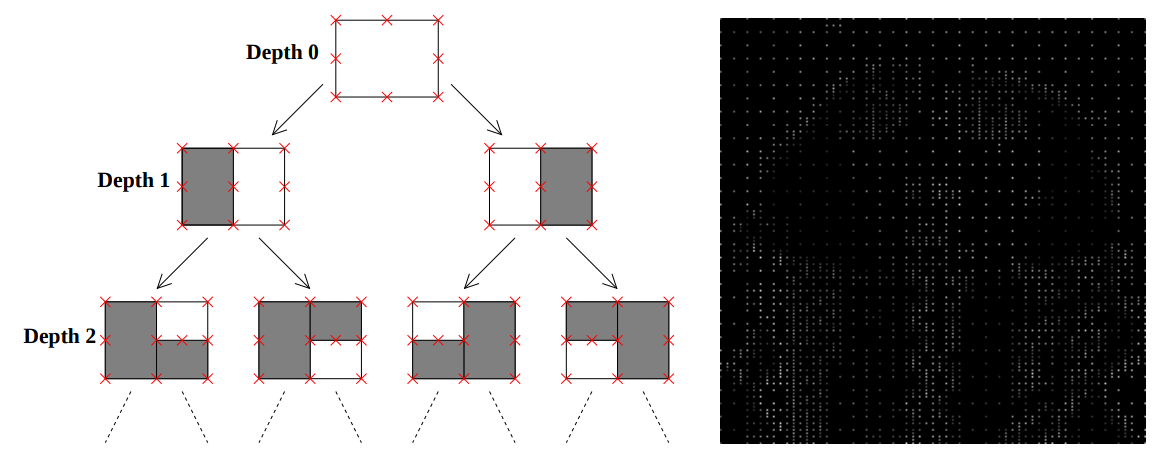
\includegraphics[width=0.8\linewidth]{tree_trui.png}
    \caption{Examples for rectangular subdivision in the R-EED codec~\cite{schmaltz09}.}
\end{figure}
In~\cite{hoeltgen12}, an alternative approach to the rectangular subdivision used in
~\cite{schmaltz09} was proposed. They considered two different methods. First, they used the results
from~\cite{belhachmi09} to derive an \textit{analytical approach} by calculating the \textit{Laplacian of a
Gaussian} $\vert \Delta f \vert^s$ for some exponent $s>0$ and then apply electrostatic 
halftoning~\cite{electrostatic} in order to get a binary point mask.\\
The second method they proposed is called \textit{probabilistic sparsification}. It works by
iteratively selecting a set percentage of pixels from the original image into the mask,
reconstructing the image using the same inpainting operator as in the decompression step, then
calculating the reconstruction error for each pixel in the inpainting mask and then throwing out
the pixels with the largest reconstruction error. This is repeated until a predefined pixel
density in the mask is reached. However, the authors stated that this method is not guaranteed to
give an optimal solution because of its greedy nature. To improve the mask they derived in the
earlier step, they introduced the so called \textit{nonlocal pixel exchange}. It aims to solve the
problem that the greediness of the probabilistic sparsification poses, more specifically that
pixels that were removed once are not considered again at a later point in time even though they
could possibly positively influence the quality of the final mask.\\
The nonlocal pixel exchange randomly selects a subset of non-mask pixels, from which the pixel with
the largest reconstruction error is put in the mask in exchange for a random mask pixel.
If the overall reconstruction quality improves with the new mask, the mask is updated to the new
mask and serves as the initial mask for the next iteration step. If the quality deteriorates with
the new mask, the change is undone and the procedure continued.
The mask resulting from this process can only be better than the previous one by construction of
the algorithm~\cite{hoeltgen12}.
Finally, they proposed several algorithms for \textit{tonal optimisation}, i.e.\ grey value
optimisation by means of a linear least squares optimisation problem. They showed some important
mathematical properties like the uniqueness and existence of a solution for this problem and
came up with a numerical algorithm to solve the linear system of equations arising for this
optimisation problem.
Using all these optimisations, they were able to cut down the reconstruction error in terms of the
mean squared error by a significant portion and achieve a quality that has not been reached before 
with similar PDE based inpainting approaches for the same mask density.

\section{Image Features In Image Reconstruction}
Features such as edges and corners are very important in the field of image processing as they
provide almost all of the semantics of an image~\cite{marr82}. Therefore, feature detection has been a staple in
this field for a long time. Actually, corner and edge detection algorithms such as the ones by John Canny
and Chris Harris~\cite{harris88, canny86} are still used today. 
Despite their semantical importance, edges and corners have not had that much impact on image
compression so far.\\
\\
In 2007, Zimmer introduced a new approach using corners to compute inpainting masks for
PDE-based image compression~\cite{zimmer07}. In their approach, they used a simple corner detection method to
sample a set of the most important corners. The inpainting mask was then obtained by storing the
8-neighbourhood around each corner. In the reconstruction or inpainting phase they used a method
following the idea proposed by Bertalmio et al.~\cite{bertalmio00}. Instead of just using pure EED to
inpaint the image, they interleaved edge-enhancing diffusion with mean curvature motion in order to
improve the inpainting in regions with sparser inpainting domains. \\
Even though their codec was
not able to compete with widely used codecs like JPEG and JPEG2000, they proved that corners are
indeed useful for PDE based inpainting. They found the largest disadvantages to be the sparsity of
corners in images. The reasoning behind this is that because of the sparsity of corners in an
image, one has to either invest in a very sophisticated and complex inpainting mechanism to fill in
the large areas between the few detected corners \textit{or} adjust the corner detector to be more
`fuzzy'. On one hand, this leads to a denser mask and hence better results reconstruction-wise 
but on the other also creates suboptimal masks with respect to compression. Due to the fuzzy nature of the
corner detector, flat or homogeneous areas are classified as corners and therefore kept in the
mask, even though these regions could have easily been filled in by even a simple inpainting
process like linear diffusion. \\
To improve on their work, they suggested to touch on the parameter
selection for the corner detector, especially the selection of both the cornerness threshold and
integration scale used in the computation of the structure tensor since these heavily influence the
amount and quality of corners that are detected. \\
The main point of criticism for this approach is that the inaccuracy of the corner 
detector was not accounted for in the selection of the mask
pixels~\cite{conversation}. Their method of limiting the amount of mask pixels by adjusting the integration scale leads
to a fairly inaccurate localisation of the corners. The cause for this will be discussed in
a later section.
Since only a small neighbourhood of pixels around each estimated corner
location was kept, the likelihood that the actual corner is not included in the final mask
increases the larger the integration scale is chosen, as we will see in Chapter~\ref{ch:Implementation}, 
where I will also adress how to approach this problem and provide a possible solution.\\
\\
In~\cite{mainberger09, mainberger10}, the authors implemented a diffusion based reconstruction
using mainly edges as the inpainting mask. For the mask construction they used the Marr-Hildreth
edge detector~\cite{marr80} combined with \textit{hysteresis thresholding} as proposed by
Canny~\cite{canny86}.
However, they stated that they were not locked in on the Marr-Hildreth edge detector and that
others such as the classical Canny edge detector could also be used, especially for images that
contain a larger amount of blurry edges. The addition of hysteresis thresholding yielded closed and
well localised contours which they encoded using the lossless \textit{JBIG} encoding~\cite{jbig}.
To reconstruct the image from the stored contours, they used a simple linear diffusion approach
which, in this case, was good enough. For cartoon-like images, they could beat the quality of
JPEG and even the more sophisticated JPEG2000 in terms of the PSNR (peak signal to noise ratio) of the reconstructed image to the
original one. In the follow-up publication from the same authors in 2010 they introduced some 
optimisations such as different
entropy coders for the edge locations as well as an optimised method of storing the grey
values of the mask pixels. Another improvement was the use of an advanced method for solving the
linear systems arising from the inpainting problem. In contrast to the earlier publications a fast
\textit{full multigrid scheme} was implemented to speed up the decoding phase significantly to 
a point where the codec is now realtime capable.\\
\\
In~\cite{peter15}, region of interest (ROI) coding was first introduced for the R-EED codec. Previously,
it was not possible to specify certain regions of an image to be reconstructed with higher detail.
With this new contribution, they allowed the user to specify a weighting mask that is used during
the mask construction phase to adapt the mask in such a way that the specified regions would have a
denser mask than other regions. This is expecially useful in medical imaging, where some regions of
an image, e.g.\ in a CT scan of a brain region, need to be reconstructed exactly in order to prevent
false diagnoses. \\
ROI coding was not the only contribution in this publication. The authors also proposed
\textit{progressive modes} for the R-EED codec to be able to compete better with widely available codecs.
Progressive modes allow an image to be displayed in a coarse manner, e.g.\ when shown on a website
that has not fully loaded the image data yet, and gradually refine the representation as more data
becomes available. Last but certainly not least, they showed that their PDE-based codec is also
capable of realtime video decoding and playback which sets a milestone in proving the
\textit{suitability of R-EED for real-world applications}~\cite{peter15}. In their words, this
publication, or rather the extensions presented therein, mark the first step of an evolution of
PDE-based compression codecs from the proof-of-concept stage to fully grown codecs with relevance
for practical applications~\cite{peter15}.\\
\\
In~\cite{kanters05}, a method is presented that uses extrema and saddle points in the Gaussian
scale space of an image as a basis for reconstruction using a linear reconstruction scheme proposed
in~\cite{janssen05}.\\
In~\cite{weinzaepfel11}, the authors explore the reconstruction of an image using only its local
descriptors. They use a classical image indexing software to retrieve descriptors like
SIFT~\cite{sift}, then query an image database to find patches that are similar to these descriptors
retrieved from the image. These patches are then transformed to fit the geometry in the original
image and stitched together afterwards in a seamless fashion.

\section{Outline}
So far, we have reviewed some of the work that is closely related to my work and 
motivated the goal that I am tring to achieve.
To explain what exactly was done in order to achieve this goal, we first have to go over some of the
theoretical background. I will introduce basic concepts from
calculus and linear algebra (\ref{sec:Basics}) as well as some more advanced topics
like the structure tensor (\ref{sec:Structure}), diffusion processes (\ref{sec:Diffusion}) and
digital image inpainting (\ref{sec:Inpainting}).\\
In Chapter~\ref{ch:Implementation}, I will then talk about the technical details of the  
implementation, for example the discretisation used to implement the theoretical ideas from 
the previous chapter (\ref{sec:Discretisation}). 
Furthermore, I will describe the shortcomings of the approach described in~\cite{zimmer07} in more
detail and discuss a method to address these issues. In this chapter, I will also present some
additional procedures that I implemented in order to improve the selection of mask pixels. \\
Afterwards, I am going to review the experiments that were performed in order to evaluate the
approach and show some examples.\\
Last but not least in Chapter~\ref{ch:Conclusion}, I conclude the work, discuss the strengths
and shortcomings of my approach and how it could be improved in future research.
